\documentclass[t]{beamer}
\usetheme{Copenhagen}
\setbeamertemplate{headline}{} % remove toc from headers
\beamertemplatenavigationsymbolsempty

\usepackage{amsmath, array, tikz, bm, pgfplots, tcolorbox, graphicx, venndiagram, color, colortbl, xfrac}
\pgfplotsset{compat = 1.16}
\usepgfplotslibrary{statistics}
\usetikzlibrary{calc}

\title{Other Probability Distributions}
\author{}
\date{}

\AtBeginSection[]
{
  \begin{frame}
    \frametitle{Objectives}
    \tableofcontents[currentsection]
  \end{frame}
}

\begin{document}

\begin{frame} 
\maketitle
\end{frame}

\section{Solve problems involving geometric probability distributions}

\begin{frame}{Binomial vs. Geometric Distributions}
With binomial distributions, we had the following conditions:
	\begin{itemize}
		\item There are a fixed number of $n$ repeated independent trials
		\item Each trial's outcome is either a success or failure
		\item The probability of success, $p$, never changes
	\end{itemize}	
	\vspace{10pt}
\onslide<2->{We could calculate the probability of obtaining 8 heads out of 10 flips of a coin.}	\newline\\
\onslide<3->{One of these outcomes is TTHTHHHTTH.}	
\end{frame}

\begin{frame}{Binomial vs. Geometric Distributions}
With geometric distributions, we would interested in the probability of obtaining our first success (flipping a tail) after $x$ flips of the coin.	\newline\\	
\onslide<2->{To put it another way, a geometric distribution has the following property:}
\onslide<3->{\[\underbrace{FFF \cdots F}_{x-1 \text{ failures}}S\]}
\end{frame}

\begin{frame}{Geometric Distributions}
The probability of obtaining our first success after $x$ binomial experiments is given by
\[P(X=x) = (1-p)^{x-1} \cdot p\]
\end{frame}

\begin{frame}{Example 1}
A student is given a 10-question multiple choice test in which each question has 5 possible answers. What is the probability that the first question the student guesses correctly on the 4th question?	\newline\\	\pause

FFFS	

\begin{align*}
\onslide<3->{P(X = 4) &= (1-0.2)^3 (0.2)}	\\[10pt]
\onslide<4->{&= 0.1024}
\end{align*}

\onslide<5->{The student has about an 10.24\% chance of first guessing correctly on the 4th question.}
\end{frame}

\begin{frame}{Bar Graph of Example 1}
\begin{center}
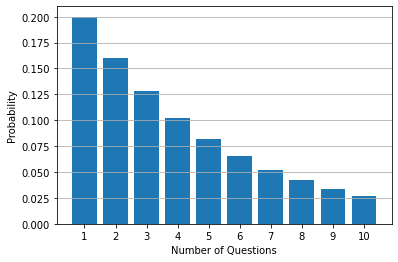
\includegraphics[scale=0.6]{../Images/geometric_mult_choice.png}
\end{center}
\end{frame}

\begin{frame}{Mean and Standard Deviation of Geometric Distributions}
The mean (expected value) of a geometric distribution is the {\color{blue}\textbf{reciprocal of the probability of success}}:

\[E(X) = \frac{1}{p}\]

\pause
The variance for a geometric distribution is the probability of failure divided by the square of the probability of success, given as 
\[\sigma^2 = \frac{1-p}{p^2}\]
\pause

From which the standard deviation, $\sigma$ is
\[\sigma = \sqrt{\frac{1-p}{p^2}} = \frac{\sqrt{1-p}}{p}\]

\end{frame}

\begin{frame}{Example 2}
(a)	\quad A student is given a 10-question multiple choice test in which each question has 5 possible answers. What is the expected number of answers a student can guess before getting one right?	\newline\\	\pause

The expected value is the reciprocal of the probability of success:
\begin{align*}
\onslide<3->{E(X) &= \frac{1}{0.2}} \\[10pt]
\onslide<4->{&= 5} 
\end{align*}

\onslide<5->{We would expect the student to answer 5 questions before guessing one correctly.}
\end{frame}

\begin{frame}{Example 2}
(b) \quad What is the standard deviation of the number of questions needed before the student guesses correctly?	\newline\\	\pause

The standard deviation is the square root of the probability of failue divided by the probability of success:
\begin{align*}
\onslide<3->{\sigma &= \frac{\sqrt{1-0.2}}{0.2}} \\[8pt]
\onslide<4->{& \approx 4.47}
\end{align*}

\onslide<5->{The standard deviation is about 4.47 questions.}
\end{frame}

\section{Solve problems involving Poisson probability distributions}

\begin{frame}{Poisson Probability Distribution}
\begin{tcolorbox}[colframe=green!20!black, colback = green!30!white,title=\textbf{Poisson Distribution}]
A \textbf{Poisson probability distribution} is a discrete probability distribution that involves occurrences of some event over a specified interval, such as time, distance, area, volume, etc.
\end{tcolorbox}
\bigskip \pause 

Poisson probability distributions have the following characteristics: 
\begin{itemize}
	\item<3->{The experiment consists of counting the number of times, $x$, an event occurs in a given interval.}
	\item<4->{The probability of the event occurring is the same for each interval.}
	\item<5->{The number of occurrences in one interval is independent of the number of occurrences in other intervals.}
\end{itemize}
\end{frame}

\begin{frame}{Poisson Formula}
\[P(X=x) = \frac{\mu^x \cdot e^{-\mu}}{x!}\]
\bigskip
where $\mu$ is the mean number of occurrences of the event over the intervals and $e \approx 2.71828$
\end{frame}

\begin{frame}{Example 3}
The mean number of dogs adopted from a rescue center per month is 4.	\newline\\	\pause
(a) \quad What is the probability that in any given month, 5 dogs will be adopted?
\begin{align*}
\onslide<3->{P(X=5) &= \frac{4^5 \cdot e^{-4}}{5!}}	\\[10pt]
\onslide<4->{&\approx 0.1563}
\end{align*}
\onslide<5->{There is about a 15.63\% chance that 5 dogs will be adopted in a given month.}
\end{frame}

\begin{frame}{Example 3}
(b) \quad What is the probability that in any given month, 2 or less dogs will be adopted?
\begin{align*}
\onslide<2->{P(X \leq 2) &= P(X=0) + P(X=1) + P(X = 2)}	\\[10pt]
\onslide<3->{&\approx 0.2381}
\end{align*}

\onslide<4->{There is about a 23.81\% chance that 2 or less dogs will be adopted in a given month.}
\end{frame}

\begin{frame}{Example 3}
(c)	\quad What is the probability that at least 3 dogs will be adopted in a given month?	
\begin{align*}
\onslide<2->{P(X \geq 3) &= 1 - P(X \leq 2)} \\[10pt]
\onslide<3->{&\approx 1 - 0.2381} \\[10pt]
\onslide<4->{&\approx 0.7619}
\end{align*}

\onslide<5->{There is about a 76.19\% chance that at least 3 dogs will be adopted in a given month.}
\end{frame}

\begin{frame}{Mean and Standard Deviation of Poisson Distributions}
The {\color{blue}\textbf{mean}} of a Poisson distribution is given to us as $\mu$, which also happens to be the variance as well.	\newline\\	\pause

Since the standard deviation is the square root of variance, it follows that the standard deviation of a Poisson distribution is also the square root of the mean:
\[\sigma = \sqrt{\mu}\]
\end{frame}
\end{document}